\begin{figure}
    \centering
    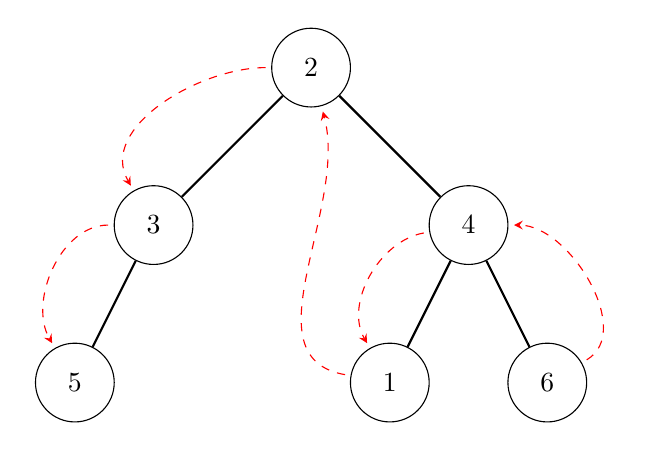
\begin{tikzpicture}[baseline=-2.25cm]
        \node[circle,draw,minimum size=1cm] (1) at (0,0)  {$2$};
        \node[circle,draw,minimum size=1cm] (2) at (-2,-2){$3$};
        \node[circle,draw,minimum size=1cm] (3) at (2,-2) {$4$};
        \node[circle,draw,minimum size=1cm] (4) at (-3,-4){$5$};
        \node[circle,draw,minimum size=1cm] (5) at (1,-4) {$1$};
        \node[circle,draw,minimum size=1cm] (6) at (3,-4) {$6$};
        \tikzstyle{filho}=[thick]
        \tikzstyle{pred}=[->, shorten >= 2pt, shorten <= 2pt,
            dashed, >=stealth, red]
        \tikzstyle{sucessor}=[->, shorten >= 2pt, shorten <= 2pt,
            dotted, >=stealth, line width=0.35mm]
        \draw[filho] (1) -- (2);
        \draw[filho] (1) -- (3);
        \draw[filho] (2) -- (4);
        \draw[filho] (3) -- (5);
        \draw[filho] (3) -- (6);
        \draw[pred] (6) edge[out=30,in=0] (3);
        \draw[pred] (3) edge[out=190,in=120] (5);
        \draw[pred] (5) edge[out=170,in=285] (1);
        \draw[pred] (1) edge[out=180,in=120] (2);
        \draw[pred] (2) edge[out=180,in=120] (4);
    \end{tikzpicture}
    \qquad
    \qquad
    \qquad
    \begin{tabular}{|c|c|c|c|}
        \hline
        $i$ & $x_0$ & $v$ & $\cert[i]$ \\
        \hline
        $1$ & $6$ & $2$ & $1$ \\

        $2$ & $3$ & $5$ & $+\infty$ \\

        $3$ & $2$ & $1$ & $2$ \\

        $4$ & $7$ & $4$ & $+\infty$ \\

        $5$ & $-2$ & $3$ & $+\infty$ \\

        $6$ & $14$ & $0.5$ & $2$ \\
        \hline
    \end{tabular}
    \caption[Representação dos certificados da ABB]{Certificados
            representados pelas setas vermelhas tracejadas. O
            certificado do elemento $5$ vale $+\infty$.}
            \label{fig:abb:cert}
\end{figure}